\documentclass[UTF8,a4paper]{ctexart}%设置a4纸和中文
\ctexset{section/format=\Large\bfseries}%设置标题左对齐
\usepackage{amsmath} % 使用align
\usepackage[margin=1in]{geometry}%设置A4值的边界
\usepackage{graphicx}%插入图片
\usepackage{amsfonts}%使用bm
\usepackage{color}
\usepackage{amssymb}
\usepackage{bm}
\author{qhy}%作者
\title{机器学习笔记4}%标题
\date{\today}%日期
\pagestyle{empty}%不显示页码
\begin{document}
  \maketitle
  \tableofcontents
  \newpage
    \section{隐马尔可夫模型 Hidden Markoy Model HMM}
        {\color{blue}
          之前我们考虑样本之间都是相互独立的,而隐马尔可夫模型则是考虑样本之间不是独立的模型。
        }
        \subsection{概率图模型}
            \textbf{概率图模型 probabilistic graphical model}是一类用图来表达变量相关关系的概率模型。
            它以图为表示工具,最常见的是用一个结点表示一个或一组随机变量,结点之间的边表示变量间的概率相关关系,即"变量关系图"。

            根据边的性质不同,概率图模型可大致分为两类:
            \begin{itemize}
              \item 有向图模型(贝叶斯网 Bayesian network)

                  使用有向无环图表示变量间的依赖关系

                  {\color{blue}
                      隐马尔可夫模型(HMM) 是结构最简单的动态贝叶斯网。
                  }

              \item 无向图模型(马尔可夫网 Markov network)

                  使用无向图表示变量间的相关关系。

            \end{itemize}
        \subsection{隐马尔可夫模型}
            马尔可夫链:系统下一时刻的状态仅由当前状态决定,不依赖以往的任何状态。

            隐马尔可夫模型是一个生成模型。

            隐马尔可夫模型中的变量可分为两组:
            \begin{itemize}
              \item 状态变量 (隐变量)

                  状态变量:$\{y_1, y_2 , \cdots , y_n\}$,其中$y_i \in \mathcal{Y} $表示第i个时刻的系统状态。\\
                  通常假定状态变量是隐藏的、不可被观测的,因此状态变量亦称\textbf{隐变量(hidden variable)}

              \item 观测变量

                  观测变量:$\{x_1, x_2 , \cdots , x_n\}$,其中$x_i \in \mathcal{X} $表示第i个时刻的观测值。
            \end{itemize}

            状态空间:$\mathcal{Y} = \{s_1,s_2,\cdots , s_N\}$,其中$s_i$表示一个具体的状态

            观测空间:$\mathcal{X} = \{o_1,o_2,\cdots , o_M\}$,其中$o_i$表示一个具体的观测值

            参数定义:$\lambda = \{\bm{A,B,\pi}\}$
            \begin{itemize}
              \item 状态转移概率

                  模型在各个状态之间转换的概率 , 通常记为矩阵 $\bm{A} = [a_{ij}]_{N\times N}$,其中
                  \[ a_{ij} = P(y_{t+1} = s_j | y_t = s_i) , 1 \leqslant i,j \leqslant N , {\color{red} \forall t }\]

                  表示在任意t时刻,若状态为$s_i$,则在下一个时刻状态为$s_j$的概率

              \item 输出观测概率

                  模型根据当前状态获得各个观测值的概率,通常记为矩阵$\bm{B} = [b_{ik}]_{N\times M}$,其中
                  \[ b_{ik} = P(x_t = o_k | y_t = s_i)  ,1 \leqslant i \leqslant N ,1 \leqslant k \leqslant M ,{\color{red} \forall t }\]

                  表示在任意时刻t,若状态为$s_i$,则观测值$o_j$被获取的概率

              \item 初始状态概率

                  模型在初始时刻各状态出现的概率,通常记为$\bm{\pi} = (\pi_1 , \pi_2 , \cdots ,\pi_N)$,其中
                  \[ \pi_i = P(y_1 = s_i) , 1 \leqslant i \leqslant N \]

                  表示模型初始状态为$s_i$的概率
            \end{itemize}

            图\ref{statusstransferfig}是状态转移图
            \begin{figure}[!htbp]
              \centering
              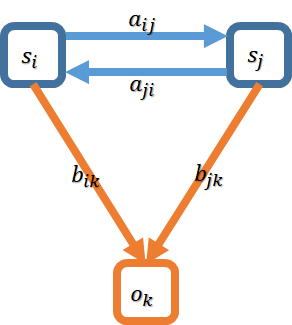
\includegraphics[scale=0.5]{assets/jiqixuexi4_85f62.png}
              \caption{状态转移图,$a_{ij}$表示从状态$s_i$转移到状态$s_j$的概率,$b{i_k}$表示状态$s_i$下观测值$o_k$被获取的概率}
              \label{statusstransferfig}
            \end{figure}

            给定状态空间$\mathcal{Y}$ , 观测空间$\mathcal{X}$ , 参数$\lambda$ , 就能确定一个隐马尔可夫模型。

            下面是给定$\lambda$下,模型产生观测序列$\{x_1, x_2, \cdots , x_n\}$的过程(见图\ref{generationOfHMM}):

            {\color{blue}
              由初始状态触发,由状态转移方程不断驱动。
            }
            \begin{itemize}
              \item [(1)] 设置$t=1$,并根据初始状态概率$\bm{\pi}$选择初始状态$y_1$
              \item [(2)] 根据状态$y_t$和观测概率$\bm{B}$选择观测变量值$x_t$
              \item [(3)] 根据状态$y_t$和状态转移矩阵$\bm{A}$转移模型状态,即确定$y_{t+1}$
              \item [(4)] 若$t<n$,设置$t=t+1$,并转到第(2)步,否则停止
            \end{itemize}

            \begin{figure}[!htbp]
              \centering
              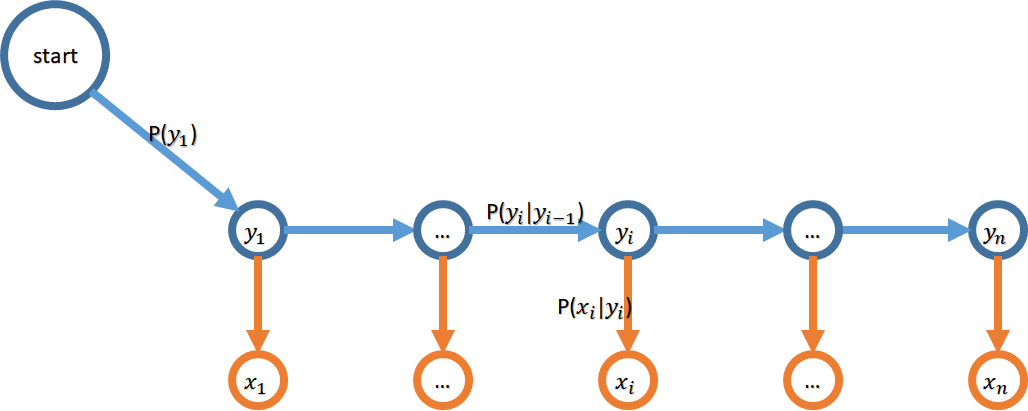
\includegraphics[scale=0.4]{assets/jiqixuexi4_06c36.png}
              \caption{隐马尔可夫模型的图结构}
              \label{generationOfHMM}
            \end{figure}

            在实际应用中,人们常关注隐马尔可夫模型的三个基本问题:
            \begin{itemize}
              \item 评估问题/预测问题
                  给定模型参数$\lambda = \{\bm{A,B,\pi}\}$,如何有效计算其产生观测序列$\{x_1, x_2, \cdots , x_n\}$ 的概率$P(\bm{x} | \lambda)$?换言之,如何评估模型与观测序列之间的匹配程度?

                  {\color{blue}
                      1. 评估模型与观测序列匹配程度:判断赌场骰子是否被动手脚\\(这里假设有多个骰子,隐变量是选择了哪个骰子,每个骰子选中的概率一样,虽然这个隐变量实际上并没有什么作用,但却和隐马尔可夫模型建立了关系,可以用隐马尔可夫模型求解)\\
                      2. 给定$\{x_1, x_2, \cdots , x_{n-1}\}$预测$x_n$,即在不同$x_n$下,求$P(\bm{x} | \lambda)$,取概率最大的$x_n$,即
                          \[ x_n^* = arg \max_{x_n} P(\bm{x} | \lambda) \]
                  }

              \item 解码问题

                  给定模型参数$\lambda = \{\bm{A,B,\pi}\}$和观测序列$\{x_1, x_2, \cdots , x_n\}$,如何找到与此观测序列最匹配的状态序列$\{y_1,y_2 , \cdots , y_n\}$?换言之,如何根据观测序列推断出隐藏的模型状态?

                  {\color{blue}
                      在语音识别中,观测值为语音信号,隐藏状态为文字,目标就是根据观测信号来推断最有可能的状态序列(即对应的文字)
                  }

              \item 学习问题

                  给定观测序列$\{x_1, x_2, \cdots , x_n\}$,如何调整模型参数$\lambda = \{\bm{A,B,\pi}\}$ 使得该序列出现的概率$P(\bm{x} | \lambda)$最大?换言之,如何训练模型使其能很好地描述观测数据?

            \end{itemize}


            {\color{blue}
                三个问题分别对应于观测变量$\{x_1,x_2,\cdot x_n\}$,状态变量$\{y_1,y_2 , \cdots , y_n\}$和参数$\lambda = \{\bm{A,B,\pi}\}$
            }

        \subsection{基本问题1-评估问题}
            给定模型参数$\lambda = \{\bm{A,B,\pi}\}$,如何有效计算其产生观测序列$\{x_1, x_2, \cdots , x_n\}$(简记为$\bm{x} = x_{1:n}$) 的概率$P(\bm{x} | \lambda)$?换言之,如何评估模型与观测序列之间的匹配程度?

            首先,在已知$\bm{y} = y_{1:n} = \{y_1, y_2 , \cdots , y_n \}$时的概率:

            {\color{blue}
              状态$x_{1:n}$由$x_{1:n-1}$经过$y_{n-1}\to y_{n} \to x_{n}$两步得到。
            }
            \begin{equation}\begin{split}
              P(\bm{x,y}|\lambda) &= P(x_{1:n},y_{1:n} | \lambda)\\
              &= P(x_{1:n-1},y_{1:n-1} | \lambda)P(y_{n}|y_{n-1})P(x_n|y_{n})\\
              &= P(y_1)P(x_1|y_1)\prod_{i = 2}^n P(y_{i}|y_{i-1})P(x_i|y_{i})
            \end{split}\end{equation}

            为方便,记$P(y_1|y_0) = P(y_1)$($y_0$不存在),则上面公式可以写成:
            \begin{equation}
              P(\bm{x,y}|\lambda) = \prod_{i = 1}^n P(y_{i}|y_{i-1})P(x_i|y_{i})
            \end{equation}

            则由全概率公式
            \begin{equation}\begin{split}
                P(\bm{x}|\lambda) &= \sum_{\bm{y}}P(\bm{x,y}|\lambda) \\
                &= \sum_{\bm{y}} \prod_{i = 1}^n P(y_{i}|y_{i-1})P(x_i|y_{i})
            \end{split}\end{equation}

            求$P(\bm{x,y}|\lambda)$耗时$O(n)$,而$\bm{y}$由$N^n$种组合,

            则计算 $P(\bm{x}|\lambda)$的时间代价为{\color{red}$O(nN^n)$},指数复杂度,显然是不可接受的

            下面介绍计算$P(\bm{x}|\lambda)$的有效算法:前向算法/后向算法

            {\color{blue}
                前向算法的本质是动态规划算法。

                而前向算法和后向算法则是同一种动态规划算法在不同方向上的实现。
            }

            \begin{itemize}
              \item 前向算法

                  \textbf{定义(前向概率)}:给定隐马尔可夫模型的参数$\bm{\lambda}$,到$t$时刻的观测序列为$\{x_1,x_2 , \cdots , x_t\}$(简记为$x_{1:t}$),时刻$t$的状态为$s_i$,定义$t$时刻的前向概率为:
                  \begin{equation}
                    \alpha_t(i) = P(x_{1:t},y_t = s_i|\bm{\lambda})
                  \end{equation}

                  则$t+1$时刻的前向概率为:
                  \begin{equation}
                    \alpha_{t+1}(i) = \left ( \sum_{j =1}^N \alpha_t(j)P(y_{t+1} = s_i|y_t = s_j) \right ) P(x_{t+1}|t_{t+1})
                  \end{equation}

                  初始条件:
                  $\alpha_1(i) = \bm{\pi_i}$

                  则序列$\{x_1,x_2 , \cdots , x_n\}$的概率就是时刻$n$的所有前向概率之和:
                  \begin{equation}
                    P(\bm{x}|\lambda = \sum_{i = 1}^N \alpha_n(i))
                  \end{equation}

              \item 后向算法

                  \textbf{定义(后向概率)}:给定隐马尔可夫模型的参数$\bm{\lambda}$,时刻$t$的状态为$s_i$,从$t+1$时刻到最后时刻$n$的部分观测序列为$\{x_{t+1},x_{t+2} , \cdots , x_n\}$(简记为$x_{t+1:n}$),则时刻t的后向概率为:
                  \begin{equation}
                    \beta_t(i) = P(x_{t+1:n}|x_t = s_i , \bm{\lambda})
                  \end{equation}

                  则$t-1$时刻的后向概率为:
                  \begin{equation}
                    \beta_{t-1}(i) = \sum_{j = 1}^N \beta_{t}(j)P(y_{t} = s_j|y_{t-1} = s_i)P(x_{t-1}|y_{t-1} = s_i)
                  \end{equation}

                  初始条件:
                  $\beta_n{i} = 1,\forall i \leqslant N$

                  则序列$\{x_1,x_2 , \cdots , x_n\}$的概率就是时刻$0$的所有后向概率之和:
                  \begin{equation}
                    P(\bm{x}|\lambda = \sum_{i = 1}^N = \pi_iP(x_1|y_1 = s_i)\beta_1(i))
                  \end{equation}

            \end{itemize}


        \subsection{基本问题2-解码问题}
        \subsection{基本问题3-学习问题}




\end{document}
